\section{THE BOX-JENKINS METHODOLOGY}

The Box-Jenkins Methodology is a three stage method for selecting an appropriate model for the purpose of estimating and forecasting a univariate time series. The model forecasts future values based on a combination of past observations (AR) and past shocks (MA). A generalization of this type of model is called SARIMA, which stands for Seasonal Autoregressive Integrated Moving Average. 

A time series $\{X_t|t=1,2,...,N\}$ is generated by a SARIMA$(p,d,q)(P,D,Q)$ process if:

$$\varphi(B)\Phi(B^S)(1-B)^d(1-B^S)^DX_t=\Theta(B)\vartheta(B^S)\epsilon_t$$     

where N is the number of observations, p, d, q, P, D and Q are integers; B is the lag operator; s is the seasonal period length.

$\varphi(B)=1-\varphi_1B - \varphi_2B^2-...-\varphi_pB^p$ is the regular autoregressive operator (AR) of order p,

$\Phi(B^S)=1-\Phi_1B - \Phi_2B^{2S}-...-\Phi_PB^P$ is the sea autoregressive operator (AR) of order P,

$\Theta(B)=1-\Theta_1B - \Theta_2B^2-...-\Theta_qB^q$ is the regular moving average operator (MA) of order q,

$\vartheta(B^S)=1-\vartheta_1B^S - \vartheta_2B^{2S}-...-\vartheta_QB^Q$ is the seasonal moving average operator (MA) of order Q,

d is the number of regular differences; D is the number of seasonal differences; $\epsilon_t$ is the residual at time $t$, identically and independently distributed with mean equal to zero and constant variance. 

The stages in the Box-Jenkins Methodology are the following:
\begin{enumerate}
\item Identification: verify the stationarity of the series and select the most relevant combination of auto-regression and moving-average. Several plausible models may appear;
\item  Estimation: the parameters of  each of the models are estimated; 
\item Diagnostic checking: ensure that the residuals of the estimated model are white noise. 
\end{enumerate}

The methodology only applies to time series that are stationary. Stationary series are series that have constant mean, constant variance, and an auto-correlation that only depends on the lag of two periods. Therefore, the first step is to test if the series is stationary. 

\subsection{Identification}

Stationary series are series that have constant mean, constant variance, and an auto-correlation that only depends on the lag between two periods. To check if the series is stationary we can make a visual inspection by looking at its plot, analyzing the ACF (Auto-correlation Function) plot, and performing unit root tests (such as the Augmented Dickey-Fuller (ADF) and the Phillips-Peron).

The ACF plot of the series (Figure \ref{fig:raw_series_plot_acf}) shows auto-correlations persisting over time, a signature of non-stationary series. Moreover, the series appears to have an upward trend up to the month of August and a downward one from September on.  This is the result of the annual seasonality which is not captured by this series. The consequence is that the mean has different values across time (i.e. it is not constant). What does appear in the series is its weekly seasonality, typical of electricity use series. The series can usually be detrended by applying its first difference. We will then be looking at changes in peak electricity consumption per day. As for the weekly seasonality, this could be captured by the first order difference If it’s not, then a seasonal difference may have to be applied. 

\begin{figure}[!htb]
\begin{center}
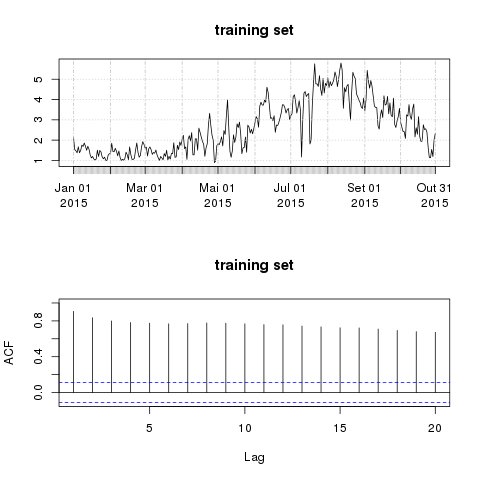
\includegraphics[width=8.4cm]{raw_series_plot_acf.png}    % The printed column width is 8.4 cm.
\caption{Plot and ACF of the raw data} 
\label{fig:raw_series_plot_acf}
\end{center}
\end{figure}


\subsubsection{Unit root test}Even though the plot and the ACF appoint to a non-stationary series, we will check if it contains a unit root by performing the Augmented Dickey Fuller Test (ADF) and Phillips-Perron test. 

The ADF test (Said and Dickey, 1984) evolved from the Dickey Fuller Test (DF), in which the null-hypothesis is that $\alpha<1$ for  the model $x_t=\alpha x_{t-1}+u_t$ in which $u_t$ is white noise. The ADF allows the differenced series $u_t$ to be any stationary process rather than only white noise. If $\alpha>1$ the series explodes and does not return to the mean (i.e. non-stationary). The test resulted in a Dickey-Fuller value of -1.446 with a p-value equal to 0.8098. The p-value is not statistically significant, therefore the null-hypothesis cannot be rejected. 
39.906

The Phillips-Perron test is different than the the ADF because it estimates the auto-correlations directly instead of approximating it with an auto-regressive model. The result of the test is a Dickey-Fuller Z(alpha) equal to -39.906 with a p-value less than 0.01. The ADF and Phillips-Perron appoint different results for the stationarity of the series. Since at least one of them (ADF) indicates non-stationarity, the null-hypothesis cannot be rejected and the series is assumed to be non-stationary. 

\subsubsection{First order difference}
The first order difference $(1-B)$ of the series (Figure \ref{fig:first_difference_acf}) is taken to try to eliminate non-stationarity. Moreover, from now on we will be working with the log of the series to account for the change in variance across time.  After the first order difference is taken, the series appears to have constant mean. To verify this hypothesis the ADF and the Phillips-Perron tests are performed: ($Dickey-Fuller=-10.901; p-value=0.01$), ($Dickey-Fuller Z(alpha)=276.18; p-value=0.01$). Both test indicate that the first order difference of the series is stationary at 1\% significance level. 

\begin{figure}[!htb]
\begin{center}
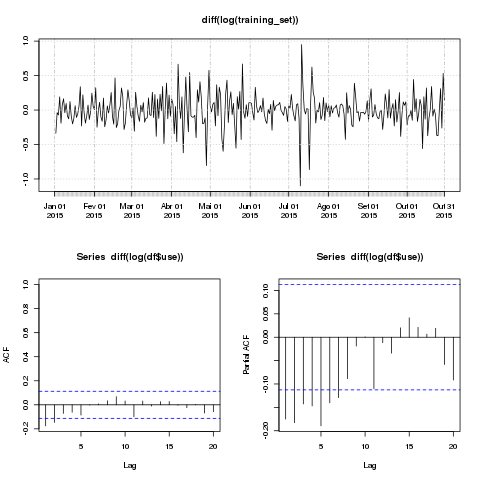
\includegraphics[width=8.4cm]{first_difference_acf.png}    % The printed column width is 8.4 cm.
\caption{Plot and ACF of the series first order difference} 
\label{fig:first_difference_acf}
\end{center}
\end{figure}

 
\subsubsection{Adding a seasonal difference}
Even though the first order difference of the series is stationary, it might not be capturing the weekly seasonality of the data. Therefore, a seasonal difference $(1-B^7)$ with a period equal to seven is applied in addition to the first order difference. This way it will have a first difference and a seasonal difference. What we are looking at now is the variation of the change in electricity consumption  per week.  The ADF and the Phillips-Perron tests for the seasonally differenced series also appoints to a stationarity at 1\% significance level ($Dickey-Fuller = -13.035, p-value = 0.01$), ($Dickey-Fuller Z(alpha) = -291.47, p-value = 0.01$)

\subsubsection{Identification of the terms that fit the series}
Now that we have the series stationary, it is possible to identify the the order of the terms (AR(p),MA(q),SAR(P) and SMA(Q)) that best describe the behavior of the series. To accomplish this, let's start by looking at the auto-correlations of the series with only the first order difference (Figure \ref{fig:first_difference_acf})

The ACF shows significant auto-correlations at lags 1 and 2. The fact that they are negative and that they “cutoff” after lag 2 is an indication that is the series is overly-differenced (i.e., a pattern of changes of sign from one observation to the next) and is suited for an MA model. Adding MA terms can partially “cancel” an order of difference in the series, correcting for over-differentiation. Moreover, this kind of model has short term memory. Specifically,  in an MA-2 process the forecast in of a given period is only dependent on the last two forecast errors (shocks). The last forecast is adjusted in the direction of the error it made. If the error was positive, i.e. if the previous forecast was too low, then the next forecast is adjusted upward by a fraction of that error. Therefore a potential model for the series is an ARIMA$(0,1,2)$. This kind of model is equivalent to a Simple Exponential Smoothing. 

Let's now look at the series with the additional seasonal difference to see what type of information can be extracted.  The plot of the seasonally differenced series (Figure \ref{fig:seasonal_difference_acf}) resembles a moving average process due to a rapid mean reverting behavior of the series.  The ACF plot confirms this. The negative auto-correlations at lags 1 and 2 and significant partial auto-correlation at lag 3 are signature of an MA(2) process. Moreover, the presence of a significant negative auto-correlation and negative partial auto-correlation at multiples of the seasonal period are signature of and SMA(1). Therefore, a good fit for the series could also be a SARIMA$(0,1,2)(0,1,1)_7$.

\begin{figure}[!htb]
\begin{center}
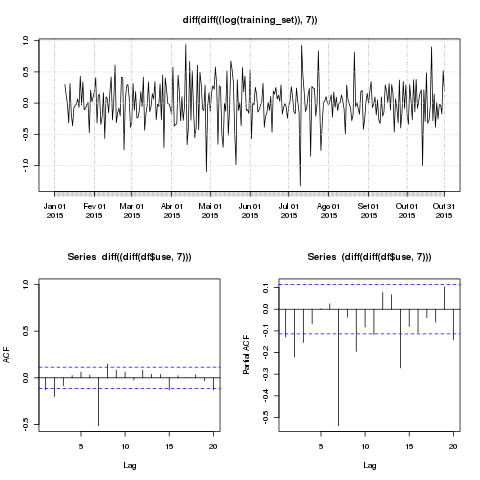
\includegraphics[width=8.4cm]{seasonal_difference_acf.png}    % The printed column width is 8.4 cm.
\caption{Plot and ACF of the seasonal and first difference} 
\label{fig:seasonal_difference_acf}
\end{center}
\end{figure}

\subsection{Estimation}
In this stage of the methodology, the parameters $\varphi, \phi, \vartheta,\Theta$ for each model are estimated by maximizing the likely-hood function (the probability of obtaining the data given the model). The fit of the models can be compared on the basis of the Akaike Information Criteria (AIC) that penalizes models with too many parameters:
$$\mathrm{AIC} = 2k - 2\ln(L) $$

In which $k$ equals the log-likelihood and $L$ the number of parameters. The lower the value of AIC the better the fit of the model to the series. 

The estimation of the parameters for the chosen models are the following: 

{\bf ARIMA(0,1,2):}

$(1-B)X_t=(1+0.39B +0.34B^2)\epsilon_t$; 

$AIC=-63.03 $; $BIC=-51.89$; $\sigma^2=0.047$

{\bf ARIMA(1,1,2):}

$(1-0.37B)(1-B)X_t=(1+0.72B +0.13B^2)\epsilon_t$; 

$AIC=-67.78$; $BIC=-52.92$; $\sigma^2=0.04$
 
{\bf SARIMA(0,1,2)(0,1,1)[7]:}

$(1-B)X_t=(1+0.39B +0.33B^2)(1-B^7)\epsilon_t$; 

$AIC=-53.44  $
$BIC=-38.6$; $\sigma^2=0.48$

{\bf SARIMA(1,1,2)(0,1,1)[7]:}

$(1-0.36B)(1-B)X_t=(1+0.71B +0.14B^2)(1-0.99B^7)\epsilon_t$; 

$AIC=-31.64$; $BIC=-13.19$; $\sigma^2=0.047$

The most parsimonious is ARIMA(1,1,2) and the least,SARIMA(1,1,2)(0,1,1)[7].
\subsection{Validation}
This stage of the methodology is about diagnostic checking the residuals of the fitted models. The closer they resemble a white noise process, the better they are at capturing the the signal from the original series and hence forecasting. We are looking to find a model fit with the following characteristics:
\begin{enumerate}
\item An ACF of the residuals that has virtually no significant values;
\item Normality of the residuals; and
\item Non-significant values of the Llung-Box Statistic
\end{enumerate}

\subsubsection{ARIMA(0,1,2)}The ACF (Figure \ref{fig:residuals_model1}) shows only two significant auto-correlations, They could be duo to chance since at least one in 20 of the auto-correlations are expected to be significant out of randomness. We could say the residuals are white noise, but the p-values for the  Lung-Box Statistic tell a different story. The null-hypothesis that the combined auto-correlation up to lag 12 is zero cannot be rejected.  This indicates that there is still information to extract from the series. The series seems to have a persistent memory up to lag 12 that the MA terms cannot capture. This could be taken into account by adding an AR term.  Also, the Q-Q plot indicates that the residuals follow a normal distribution expect for extreme values. 

\begin{figure}[!htb]
\begin{center}
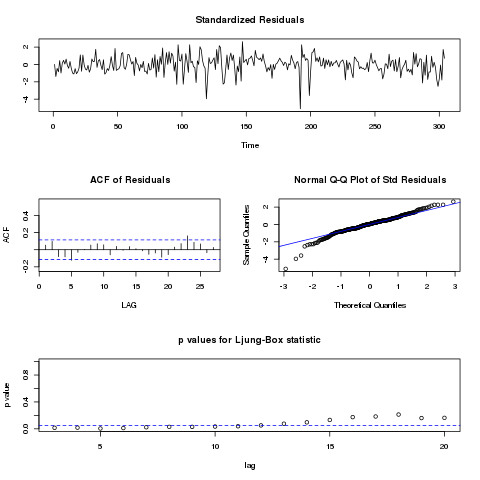
\includegraphics[width=8.4cm]{residuals_model1.png}    % The printed column width is 8.4 cm.
\caption{Residual analysis of ARIMA(0,1,2)} 
\label{fig:residuals_model1}
\end{center}
\end{figure}

                   

\subsubsection{ARIMA(1,1,2)}

Adding an AR term to the previous model compensates for  a possible under-differentiation.  It will make the forecast of a period $t$ dependent on a fraction of $t_{-1}$ (including the error term).  While an MA(1) will be only of the forecast error (the shock). In essence and AR model, a shock will have permanent effects on the series, while in an MA(k) model only for the k periods. When we add AR terms we are adding “memory” to the series.  
Adding an AR term lowered the standard error of the residuals and the AIC of the model.  The residuals have only 1 significant auto-correlation (Figure \ref{fig:residuals_model2}), which is expected to happened by chance in a 25 period ACF. The residuals follow a normal distribution expect on extreme values (outliers). The significant difference with the ARIMA(0,1,2) is in the Lung-Box Statistic, which now shows no significant auto-correlation up to any lag. This means that by adding an AR(1) we were able to capture more “signal” from the series and leave only the “noise”. In other words, the ARIMA(0,1,2) was trying to model a rapid mean reverting behavior, while the original series has a slower one. 
\begin{figure}[!htb]
\begin{center}
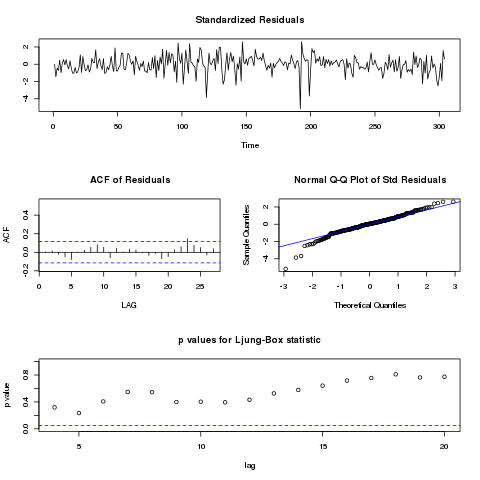
\includegraphics[width=8.4cm]{residuals_model2.png}    % The printed column width is 8.4 cm.
\caption{Residual analysis of ARIMA(1,1,2)} 
\label{fig:residuals_model2}
\end{center}
\end{figure}


\subsubsection{SARIMA(0,1,2)(0,1,1)}The AIC value is larger than for the model with only a first difference. Let’s take a look at the residuals. The ACF shows (Figure \ref{fig:residuals_model3})two significant spikes, they could be due to chance as they are small in value (less than 0.2). The problem lies in Ljung-Box statistic, telling us that the null hypothesis that all the auto-correlation up to lag 15 are zero cannot be rejected. This implies that there is some pattern that the model is not recognizing. It is possible that by including an AR term in the non-seasonal part this signal could be captured. 

\begin{figure}[!htb]
\begin{center}
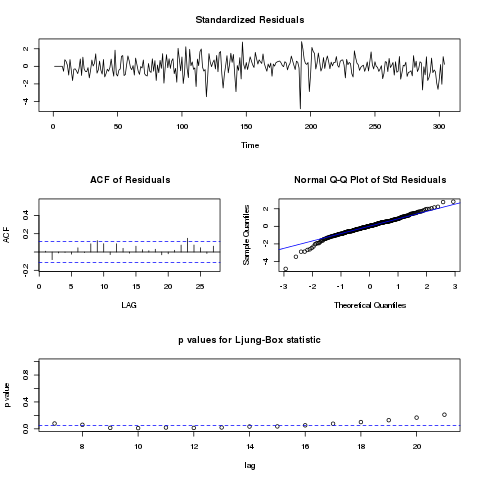
\includegraphics[width=8.4cm]{residuals_model3.png}    % The printed column width is 8.4 cm.
\caption{Residual analysis of SARIMA(0,1,2)(0,1,1)[7]} 
\label{fig:residuals_model3}
\end{center}
\end{figure}

\subsubsection{SARIMA(1,1,2)(0,1,1)} This model has only one significant value of auto-correlation, which is to be expected in 20 lags. The residuals resemble a normal distribution, again except outliers. The significant difference that the addition of an ordinary AR(1) term brought is the values for the Llung-Box statistic. The values are all bellow the significance level and thus the residuals of this model fit are purely white noise. This makes it a good candidate for forecasting. 

\begin{figure}[!htb]
\begin{center}
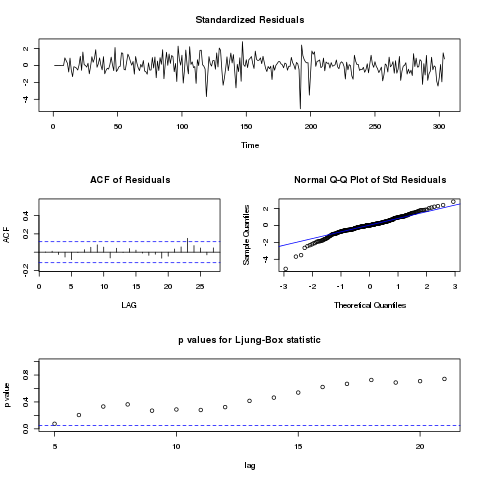
\includegraphics[width=8.4cm]{residuals_model4.png}    % The printed column width is 8.4 cm.
\caption{Residual analysis of SARIMA(1,1,2)(0,1,1)[7]} 
\label{fig:residuals_model4}
\end{center}
\end{figure}

\subsection{Forecasting}
With the fitted models validated, the next step in the methodology is to use them for forecasting and measure their accuracy. The forecasts are dynamic,in the sense that out-of-sample values are updated. The forecast plots (shown only the out-of-sample values) are in Figure \ref{fig:forecast_all}. The gray line represents the observed data and the black, the forecast. 

Two forecast measures are used, Root Mean Square Error(RMSE) and Mean Absolute Percentage Error(MAPE). Their values for each model is are in Table \ref{tb:accuracy}. 

\begin{table}[!hb]
\begin{center}
\caption{Forecast accuracy}\label{tb:accuracy}
\begin{tabular}{cccc}
Model & RMSE & MAPE  \\\hline
ARIMA(0,1,2) & 	0.327 & 17.25 \\
ARIMA(1,1,2) & 0.321 & 16.789 \\
SARIMA(0,1,2)(0,1,1)[7] & 0.304 & 15.63  \\
SARIMA(1,1,2)(0,1,1)[7] & 0.296 & 15.00  \\ \hline
\end{tabular}
\end{center}
\end{table}

The model with the lowest RMSE and MAPE is the SARIMA(1,1,2)(0,1,1)[7]. 
\begin{figure*}[!htb]
\begin{center}
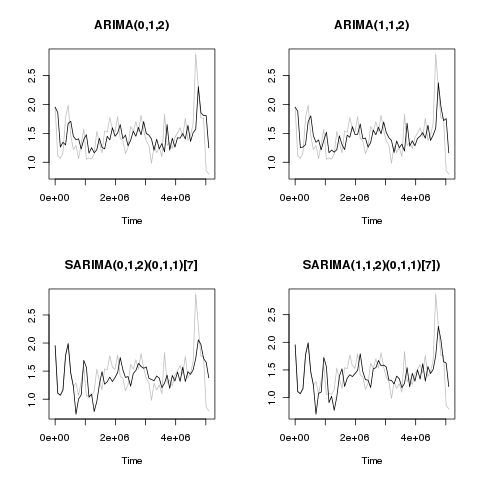
\includegraphics[width=\textwidth]{forecast_all.png}    % The printed column width is 8.4 cm.
\caption{Forecast of the models} 
\label{fig:forecast_all}
\end{center}
\end{figure*}